\section{Model selection}

%%%%%%%%%%%%%%%%%%%%%%%%%%%%%%%%%%%%

\subsection{Identifying significance}

%%%%%%%%%%%%%%%%%%%%%%%%%%%%%%%%%%%

\begin{frame}
\frametitle{Beauty in the classroom}

\begin{itemize}

\item Data: Student evaluations of instructors' beauty and teaching quality for 463 courses at the University of Texas.

\item Evaluations conducted at the end of semester, and the beauty judgements were made later, by six students who had not attended the classes and were not aware of the course evaluations (2 upper level females, 2 upper level males, one lower level female, one lower level male).

\end{itemize}

\ct{Hamermesh \& Parker. (2004)``Beauty in the classroom: instructors� pulchritude and putative pedagogical productivity� Economics Education Review.}

\end{frame}

%%%%%%%%%%%%%%%%%%%%%%%%%%%%%%%%%%%

\begin{frame}
\frametitle{Professor rating vs. beauty}

Professor evaluation score (higher score means better) vs. beauty score (a score of 0 means average, negative score means below average, and a positive score above average):

\begin{center}
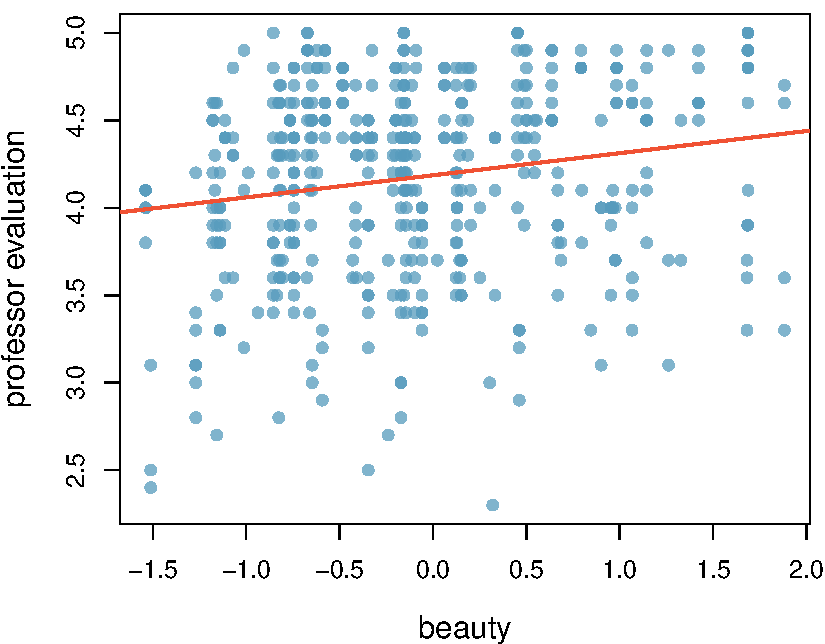
\includegraphics[width=0.65\textwidth]{8-2_model_select/figures/beauty/beauty_profeval}
\end{center}

\end{frame}

%%%%%%%%%%%%%%%%%%%%%%%%%%%%%%%%%%%

\begin{frame}
\frametitle{}

\pq{Which of the below is \underline{correct} based on the model output?}

\begin{center}
{\small
\begin{tabular}{rrrrr}
  \hline
 & Estimate & Std. Error & t value & Pr($>$$|$t$|$) \\ 
  \hline
(Intercept) & 4.19 & 0.03 & 167.24 & 0.00 \\ 
  beauty & 0.13 & 0.03 & 4.00 & 0.00 \\
   \hline
$R^2$ = 0.0336
\end{tabular}
}
\end{center}

\begin{enumerate}[(a)]
\item Model predicts 3.36\% of professor ratings correctly.
\item Beauty is not a significant predictor of professor evaluation.
\solnMult{Professors who score 1 point above average in their beauty score are tend to also score 0.13 points higher in their evaluation.}
\item 3.36\% of variability in beauty scores can be explained by professor evaluation.
\item The correlation coefficient could be $\sqrt{0.0336} = 0.18$ or $-0.18$, we can't tell which is correct.
\end{enumerate}

\end{frame}

%%%%%%%%%%%%%%%%%%%%%%%%%%%%%%%%%%%

\begin{frame}
\frametitle{Exploratory analysis}

\twocol{0.4}{0.6}
{
\dq{Any interesting features?}
\soln{\only<2->{Few females with very low beauty scores.}}
$\:$ \\
\dq{For a given beauty score, are male professors evaluated higher, lower, or about the same as female professors?}
\soln{\only<3->{Difficult to tell from this plot only.}}
}
{
\begin{center}
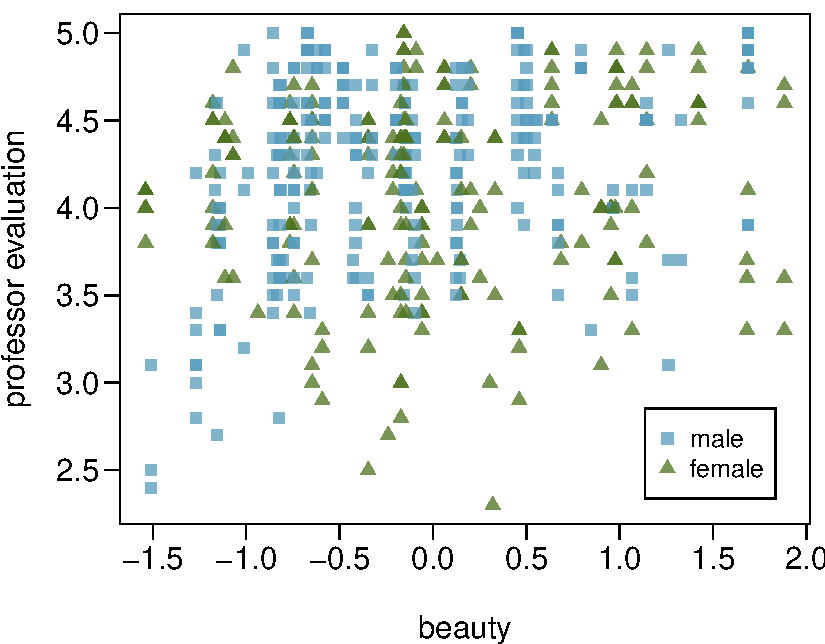
\includegraphics[width=\textwidth]{8-2_model_select/figures/beauty/beauty_profeval_gender}
\end{center}
}

\end{frame}

%%%%%%%%%%%%%%%%%%%%%%%%%%%%%%%%%%

\begin{frame}[fragile]
\frametitle{Professor rating vs. beauty + gender}

\pq{For a given beauty score, are male professors evaluated higher, lower, or about the same as female professors?}

{\small
\begin{center}
\begin{tabular}{rrrrr}
  \hline
 & Estimate & Std. Error & t value & Pr($>$$|$t$|$) \\ 
  \hline
(Intercept) & 4.09 & 0.04 & 107.85 & 0.00 \\ 
  beauty & 0.14 & 0.03 & 4.44 & 0.00 \\ 
  gender.male & 0.17 & 0.05 & 3.38 & 0.00 \\ 
   \hline
$R^2_{adj}$ = 0.057
\end{tabular}
\end{center}
}

\begin{enumerate}[(a)]
\solnMult{higher} \soln{\only<2>{\red{$\rightarrow$ Beauty held constant, male professors are rated 0.17 points higher on average than female professors.}}}
\item lower
\item about the same
\end{enumerate}

\end{frame}

%%%%%%%%%%%%%%%%%%%%%%%%%%%%%%%%%%%

\begin{frame}[fragile]
\frametitle{Full model}

{\small
\begin{center}
\begin{tabular}{rrrrr}
  \hline
 & Estimate & Std. Error & t value & Pr($>$$|$t$|$) \\ 
  \hline
(Intercept) & 4.6282 & 0.1720 & 26.90 & 0.00 \\ 
  beauty & 0.1080 & 0.0329 & 3.28 & 0.00 \\ 
  gender.male & 0.2040 & 0.0528 & 3.87 & 0.00 \\ 
  age & -0.0089 & 0.0032 & -2.75 & 0.01 \\ 
formal.yes \footnote{\texttt{formal}: picture wearing tie\&jacket/blouse, levels: \texttt{yes}, \texttt{no}} & 0.1511 & 0.0749 & 2.02 & 0.04 \\ 
  lower.yes \footnote{\texttt{lower}: lower division course, levels: \texttt{yes}, \texttt{no}} & 0.0582 & 0.0553 & 1.05 & 0.29 \\ 
  native.non english & -0.2158 & 0.1147 & -1.88 & 0.06 \\ 
  minority.yes & -0.0707 & 0.0763 & -0.93 & 0.35 \\ 
  students \footnote{\texttt{students}: number of students} & -0.0004 & 0.0004 & -1.03 & 0.30 \\ 
  tenure.tenure track \footnote{\texttt{tenure}: tenure status, levels: \texttt{non-tenure track}, \texttt{tenure track}, \texttt{tenured}} & -0.1933 & 0.0847 & -2.28 & 0.02 \\ 
  tenure.tenured & -0.1574 & 0.0656 & -2.40 & 0.02 \\ 
   \hline
\end{tabular}
\end{center}
}

\end{frame}

%%%%%%%%%%%%%%%%%%%%%%%%%%%%%%%%%%%

\begin{frame}
\frametitle{Hypotheses}

Just as the interpretation of the slope parameters take into account all other variables in the model,  the hypotheses for testing for significance of a predictor also takes into account all other variables.

$\:$ \\

\begin{itemize}
\item[] \mathhl{H_0:} $B_i = 0$ when other explanatory variables are included in the model.
\item[] \mathhl{H_A:} $B_i \ne 0$ when other explanatory variables are included in the model.
\end{itemize}

\end{frame}

%%%%%%%%%%%%%%%%%%%%%%%%%%%%%%%%%%%

\begin{frame}
\frametitle{Assessing significance: numerical variables}

\pq{The p-value for age is 0.01. What does this indicate?}

{\scriptsize
\begin{center}
\begin{tabular}{rrrrr}
  \hline
 & Estimate & Std. Error & t value & Pr($>$$|$t$|$) \\ 
  \hline
...\\
  age & -0.0089 & 0.0032 & -2.75 & 0.01 \\ 
...\\
   \hline
\end{tabular}
\end{center}
}

\begin{enumerate}[(a)]
\item Since p-value is positive, higher the professor's age, the higher we would expect them to be rated.
\solnMult{If we keep all other variables in the model, there is strong evidence that professor's age is associated with their rating.}
\item Probability that the true slope parameter for age is 0 is 0.01.
\item There is about 1\% chance that the true slope parameter for age is -0.0089.
\end{enumerate}

\end{frame}

%%%%%%%%%%%%%%%%%%%%%%%%%%%%%%%%%%%

\begin{frame}[fragile]
\frametitle{Assessing significance: categorical variables}

\pq{{\small Tenure is a categorical variable with 3 levels: non tenure track, tenure track, tenured. Based on the model output given, which of the below is \underline{false}?}}

{\footnotesize
\begin{center}
\begin{tabular}{rrrrr}
  \hline
 & Estimate & Std. Error & t value & Pr($>$$|$t$|$) \\ 
  \hline
... \\
  tenure.tenure track & -0.1933 & 0.0847 & -2.28 & 0.02 \\ 
  tenure.tenured & -0.1574 & 0.0656 & -2.40 & 0.02 \\ 
   \hline
\end{tabular}
\end{center}
}

\begin{enumerate}[(a)]
\item Reference level is non tenure track.
\item All else being equal, tenure track professors are rated, on average, 0.19 points lower than non-tenure track professors.
\item All else being equal, tenured professors are rated, on average, 0.16 points lower than non-tenure track professors.
\solnMult{All else being equal, there is a significant difference between the average ratings of tenure track and tenured professors.}
\end{enumerate}

\end{frame}

%%%%%%%%%%%%%%%%%%%%%%%%%%%%%%%%%%%

\begin{frame}
\frametitle{Assessing significance}

\dq{Which predictors do not seem to meaningfully contribute to the model, i.e. may not be significant predictors of professor's rating score?}

{\scriptsize
\begin{center}
\begin{tabular}{rrrrr}
  \hline
 & Estimate & Std. Error & t value & Pr($>$$|$t$|$) \\ 
  \hline
(Intercept) & 4.6282 & 0.1720 & 26.90 & 0.00 \\ 
  beauty & 0.1080 & 0.0329 & 3.28 & 0.00 \\ 
  gender.male & 0.2040 & 0.0528 & 3.87 & 0.00 \\ 
  age & -0.0089 & 0.0032 & -2.75 & 0.01 \\ 
  formal.yes & 0.1511 & 0.0749 & 2.02 & 0.04 \\ 
  \rowcolor{oiB!50}
  lower.yes & 0.0582 & 0.0553 & 1.05 & 0.29 \\ 
    \rowcolor{oiB!50}
  native.non english & -0.2158 & 0.1147 & -1.88 & 0.06 \\ 
    \rowcolor{oiB!50}
  minority.yes & -0.0707 & 0.0763 & -0.93 & 0.35 \\ 
    \rowcolor{oiB!50}
  students & -0.0004 & 0.0004 & -1.03 & 0.30 \\ 
  tenure.tenure track & -0.1933 & 0.0847 & -2.28 & 0.02 \\ 
  tenure.tenured & -0.1574 & 0.0656 & -2.40 & 0.02 \\ 
   \hline
\end{tabular}
\end{center}
}

\end{frame}

%%%%%%%%%%%%%%%%%%%%%%%%%%%%%%%%%%%

\subsection{Model selection methods}

%%%%%%%%%%%%%%%%%%%%%%%%%%%%%%%%%%%

\begin{frame}
\frametitle{Model selection strategies}

\dq{Based on what we've learned so far, what are some ways you can think of that can be used to determine which variables to keep in the model and which to leave out?}

\end{frame}


%%%%%%%%%%%%%%%%%%%%%%%%%%%%%%%%%%%

\begin{frame}
\frametitle{Backward-elimination}

\begin{enumerate}

\item $R^2_{adj}$ approach: 
\begin{itemize}
\item Start with the full model
\item Drop one variable at a time and record $R^2_{adj}$ of each smaller model
\item Pick the model with the highest increase in $R^2_{adj}$
\item Repeat until none of the models yield an increase in $R^2_{adj}$
\end{itemize}

\item p-value approach: 
\begin{itemize}
\item Start with the full model
\item Drop the variable with the highest p-value and refit a smaller model
\item Repeat until all variables left in the model are significant
\end{itemize}

\end{enumerate}

\end{frame}

%%%%%%%%%%%%%%%%%%%%%%%%%%%%%%%%%%%

\begin{frame}[shrink]
\frametitle{Backward-elimination: $R^2_{adj}$ approach}

\vspace{-0.15cm}

{\tiny
\begin{tabular}{l | l | c}
\textbf{Step}		& \textbf{Variables included}	& $\mathbf{R^2_{adj}}$ \\
\hline
Full		& beauty + gender + age + formal + lower + native + minority + students + tenure & \red{0.0839} \pause \\
\hline
Step 1 	& gender + age + formal + lower + native + minority + students + tenure		& 0.0642 \\
		& beauty + age + formal + lower + native + minority + students + tenure		& 0.0557 \\
		& beauty + gender + formal + lower + native + minority + students + tenure	& 0.0706 \\
		& beauty + gender + age + lower + native + minority + students + tenure		& 0.0777 \\
		& beauty + gender + age + formal + native + minority + students + tenure		& 0.0837 \\
		& beauty + gender + age + formal + lower + minority + students + tenure		& 0.0788 \\
		& beauty + gender + age + formal + lower + native + students + tenure		& \red{0.0842} \\
		& beauty + gender + age + formal + lower + native + minority + tenure		& 0.0838 \\
		& beauty + gender + age + formal + lower + native + minority + students		& 0.0733 \pause \\
\hline		
Step 2	& gender + age + formal + lower + native + students + tenure 				& 0.0647 \\
		& beauty + age + formal + lower + native + students + tenure 				& 0.0543 \\
		& beauty + gender + formal + lower + native + students + tenure 			& 0.0708 \\
		& beauty + gender + age + lower + native + students + tenure 				&0.0776  \\
		& beauty + gender + age + formal + native + students + tenure 			& \red{0.0846} \\
		& beauty + gender + age + formal + lower + native + tenure 				& 0.0844 \\
		& beauty + gender + age + formal + lower + native + students 				& 0.0725 \pause \\
\hline
Step 3	& gender + age + formal + native + students + tenure 					& 0.0653 \\
		& beauty + age + formal + native + students + tenure					& 0.0534 \\
		& beauty + gender + formal + native + students + tenure					& 0.0707 \\
		& beauty + gender + age + native + students + tenure					& 0.0786 \\
		& beauty + gender + age + formal + students + tenure					& 0.0756 \\
		& beauty + gender + age + formal + native + tenure						& \red{0.0855} \\
		& beauty + gender + age + formal + native + students					& 0.0713 \pause \\
\hline
Step 4	& gender + age + formal + native + tenure 							& 0.0667 \\
		& beauty + age + formal + native + tenure								& 0.0553 \\
		& beauty + gender + formal + native + tenure							& 0.0723 \\
		& beauty + gender + age + native + tenure							& 0.0806 \\
		& beauty + gender + age + formal + tenure							& 0.0773 \\
		& beauty + gender + age + formal + native							& 0.0713 \\
\end{tabular}
}

\end{frame}

%%%%%%%%%%%%%%%%%%%%%%%%%%%%%%%%%%%

\begin{frame}[fragile]
\frametitle{\texttt{step} function in R}

{\scriptsize
\begin{verbatim}
Call:
lm(formula = profevaluation ~ beauty + gender + age + formal + 
    native + tenure, data = d)

Coefficients:
       (Intercept)              beauty          gendermale  
          4.628435            0.105546            0.208079  
               age           formalyes   nativenon english  
         -0.008844            0.132422           -0.243003  
tenuretenure track       tenuretenured  
         -0.206784           -0.175967  
\end{verbatim}
}

$\:$

\pause
Best model: beauty + gender + age + formal + native + tenure

\end{frame}

%%%%%%%%%%%%%%%%%%%%%%%%%%%%%%%%%%%

\begin{frame}
\frametitle{Backward-elimination: $p-value$ approach}

{\tiny
\begin{tabular}{l | rrrrrrrrrr }
\textbf{Step}		& \multicolumn{10}{c}{ \textbf{Variables included \& p-value} } \\
\hline
Full		& beauty	& gender		& age	& formal		& lower 	& native	 	& minority		& students	& tenure		& tenure \\
		& 		& male		& 		& yes		& yes	 & non english	& yes		& 			& tenure track	& tenured \\
		&  0.00 	&  0.00 		& 0.01	& 0.04		& 0.29	& 0.06		& \red{0.35}	& 0.30		& 0.02		& 0.02 \pause \\
\hline
Step 1	& beauty	& gender		& age	& formal		& lower 		& native	 	& 			& students	& tenure		& tenure \\
		& 		& male		& 		& yes		& yes		& non english	& 			& 			& tenure track	& tenured \\
		&  0.00 	&  0.00 		& 0.01	& 0.04		& \red{0.38}	& 0.03		&			& 0.34		& 0.02		& 0.01 \pause\\
\hline
Step 2	& beauty	& gender		& age	& formal		& 	 		& native	 	& 			& students	& tenure		& tenure \\
		& 		& male		& 		& yes		& 			& non english	& 			& 			& tenure track	& tenured \\
		&  0.00 	&  0.00 		& 0.01	& 0.05		& 			& 0.02		&			& \red{0.44}	& 0.01		& 0.01\pause \\
\hline
Step 3 	& beauty	& gender		& age	& formal		& 	 		& native	 	& 			& 			& tenure		& tenure \\
		& 		& male		& 		& yes		& 			& non english	& 			& 			& tenure track	& tenured \\
		&  0.00 	&  0.00 		& 0.01	& \red{0.06}	& 			& 0.02		&			& 			& 0.01		& 0.01 \pause \\
\hline
Step 	4	& beauty	& gender		& age	& 			& 	 		& native	 	& 			& 			& tenure		& tenure \\
		& 		& male		& 		& 			& 			& non english	& 			& 			& tenure track	& tenured \\
		&  0.00 	&  0.00 		& 0.01	&			& 			& \red{0.06}	&			& 			& 0.01		& 0.01 \pause \\
\hline
Step 5 	& beauty	& gender		& age	& 			& 	 		& 		 	& 			& 			& tenure		& tenure \\
		& 		& male		& 		& 			& 			&			& 			& 			& tenure track	& tenured \\
		&  0.00 	&  0.00 		& 0.01	&			& 			& 			&			& 			& 0.01		& 0.01 \\
\end{tabular}
}

$\:$ \\

\pause
Best model: beauty + gender + age + tenure

\end{frame}

%%%%%%%%%%%%%%%%%%%%%%%%%%%%%%%%%%%

\begin{frame}
\frametitle{Forward-selection}

\begin{enumerate}

\item $R^2_{adj}$ approach: 
\begin{itemize}
\item Start with regressions of response vs. each explanatory variable
\item Pick the model with the highest $R^2_{adj}$
\item Add the remaining variables one at a time to the existing model, and once again pick the model  with the highest $R^2_{adj}$
\item Repeat until the addition of any of the remanning variables does not result in a higher $R^2_{adj}$
\end{itemize}

\item $p-value$ approach: 
\begin{itemize}
\item Start with regressions of response vs. each explanatory variable
\item Pick the variable with the lowest significant p-value 
\item Add the remaining variables one at a time to the existing model, and pick the variable with the lowest significant p-value
\item Repeat until any of the remaining variables does not have a significant p-value
\end{itemize}

\textit{In forward-selection the p-value approach isn't any simpler (you still need to fit a bunch of models), so there's almost no incentive to use it.}

\end{enumerate}

\end{frame}


%%%%%%%%%%%%%%%%%%%%%%%%%%%%%%%%%%%

\begin{frame}[fragile]
\frametitle{Selected model}

\begin{center}
\begin{tabular}{rrrrr}
  \hline
 & Estimate & Std. Error & t value & Pr($>$$|$t$|$) \\ 
  \hline
(Intercept) & 4.6284 & 0.1673 & 27.66 & 0.00 \\ 
  beauty & 0.1055 & 0.0328 & 3.21 & 0.00 \\ 
  gender.male & 0.2081 & 0.0519 & 4.01 & 0.00 \\ 
  age & -0.0088 & 0.0032 & -2.75 & 0.01 \\ 
  formal.yes & 0.1324 & 0.0714 & 1.85 & 0.06 \\ 
  native:non english & -0.2430 & 0.1080 & -2.25 & 0.02 \\ 
  tenure:tenure track & -0.2068 & 0.0839 & -2.46 & 0.01 \\ 
  tenure:tenured & -0.1760 & 0.0641 & -2.74 & 0.01 \\ 
   \hline
\end{tabular}
\end{center}

\end{frame}
